\documentclass[fontsize=28pt,a4paper]{scrartcl}

\usepackage[margin=0.75in,includefoot,bottom=0.3in,footskip=2em]{geometry}

\usepackage{fontspec}
\setmainfont{EBGaramond}
[
  Extension      = .otf,
  UprightFont    = *-Regular,
  ItalicFont     = *-Italic,
  BoldFont       = *-Bold,
  BoldItalicFont = *-BoldItalic,
  Numbers        = Lowercase,
  Ligatures      = Discretionary,
  Style          = Swash
]
% https://texnique.fr/osqa/questions/8423/lualatex-et-ligatures

\usepackage[french]{babel}

% https://tex.stackexchange.com/a/123669/295527
%\renewcommand*{\FrenchLabelItem}{$\bullet$}
%\frenchsetup{StandardItemLabels=true}
\frenchsetup{StandardLayout=true}

\usepackage{microtype}

%\usepackage{xcolor}
%\usepackage{tikz}
%\usetikzlibrary{intersections,calc}
%\usepackage{caption}

\usepackage[showmarks]{pocketmod}% https://github.com/liantze/pocketmod.sty

\usepackage{graphicx}
\usepackage{enumitem}
\setlist{leftmargin=\parindent,labelindent=*}
\usepackage{hyperref}
\usepackage[hyphenbreaks]{breakurl}

\usepackage{caption}
\usepackage{longtable,booktabs,array}

\title{La justice}

\author{\small R. Chastain}
\date{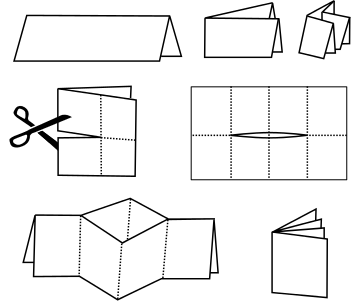
\includegraphics[width=.75\textwidth]{folding-minibook}}

\begin{document}

\maketitle
\thispagestyle{empty}
\clearpage

%La réponse de Céphale (à la question de savoir quel est l'avantage d'avoir de l'argent) n'est pas la réponse de tout le monde. Il y a une crainte que connaissent les vieillards et que ne connaissent pas les jeunes gens. Il s'agit de ce qu'on raconte au sujet de l'enfer : au sujet des châtiments qui seraient réservés dans l'au-delà, à ceux qui ont commis des injustices dans cette vie. Les jeunes, en général, se moquent de ces histoires, qu'ils prennent pour des fables. Les vieux, au contraire, craignent que ces histoires ne soient vraies. Ceux qui se savent innocents  passent leurs vieux jours dans l'espérance, tandis que les autres les passent dans la crainte. C'est là que le vrai avantage de la richesse apparaît. L'homme riche peut payer ses dettes. L'homme pauvre est quelquefois contraint de commettre des injustices, par exemple s'il n'a pas de quoi payer ses dettes. (À comparer avec la définition du courage par Lachès.) Voilà donc la plus grande utilité de l'argent selon Céphale.
%Socrate pose alors la question de l'essence de la justice. Pour Céphale, la justice consiste à rendre chacun ce qui lui appartient. N' y a-t-il pas certaines circonstances où il est injuste de rendre à quelqu'un ce qui lui appartient ? Par exemple un ami m'a confié une arme, alors qu'il était sain d'esprit. Devenu fou, il vient me la réclamer. Tout le monde conviendra qu'on ne doit pas lui rendre son arme, que ce ne serait pas juste.
%La définition, que Céphale a proposée, de la justice n'est pas satisfaisante.
%La plupart des vieilles gens regrettent les plaisirs de la jeunesse, les plaisirs des sens. Ils estiment qu'une vie sans plaisir est une vie malheureuse. On appelle *hédonisme* cette philosophie qui assimile bonheur au plaisir. On pourrait l'appeler aussi *épicurisme*, à cause d'Épicure.
%Mot de Sophocle. Sophocle s'estime heureux de ne plus éprouver ce genre de désir. Il voit dans le désir amoureux "un maître furieux et tyrannique". L'âme humaine est comme une maison, ou comme une cité.
%Richesse. Il est plus facile à l'homme riche de payer ses dettes. Soit qu'il doive un sacrifice à un dieu, soit qu'il doive de l'argent à un homme, il peut s'en acquitter (il en a les moyens). Ce qui inquiète Céphale, c'est de mourir avec des dettes. L'idée que Céphale se fait de la justice, c'est de rendre à chacun ce qui lui appartient. (Dans la prière du Notre Père, dans sa version latine, il est aussi question de dettes : "remettez-nous nos dettes commes nous remettons à nos débiteurs".) C'est l'image que Céphale se fait de la justice.
%Mais si un ami m'a confié une arme, alors qu'il était sain d'esprit, et que devenu fou, il me la réclame, je ferais une mauvaise action si je la lui rendais. Ce ne serait pas agir avec justice, ce ne serait pas bien agir. Donc la question se pose de savoir ce qu'est la justice, et comment on peut la définir.
%Il y a un auteur qui a expliqué pourquoi on ne doit pas rendre l'épée : c'est Domat dans le *Traité des lois*. Rendre l'épée dans ces circonstances, ce ne serait pas aimer la personne (vouloir son bien). Ce serait serait enfreindre le commandement d'aimer.

\subsubsection*{Payer ce qu'on doit.}

Au début de \textit{La République}, Socrate demande à son ami Céphale quel est selon lui le principal avantage de la richesse. La réponse de Céphale n'est pas celle de tout le monde. À mesure que les hommes vieillissent, dit-il, ils commencent à craindre que ce qu'on raconte, au sujet des châtiments qui attendraient dans l'au-delà ceux qui ont commis des injustices pendant leur vie, ne soit vrai. L'avantage de la richesse est qu'on peut payer ses dettes avant de mourir, soit qu'on doive un sacrifice à un dieu, soit qu'on doive de l'argent à un homme. La justice, telle que Céphale la conçoit, consiste à rendre à chacun ce qui lui appartient ou ce qu'on lui doit.

Pourtant, remarque Socrate, si un ami m'a confié une arme et que, devenu fou, il me demande de la lui restituer, ce ne serait pas agir avec justice que de la lui rendre. La définition que Céphale a donnée de la justice ne paraît donc pas suffisante. Jean Domat, dans le \textit{Traité de lois}, dira que rendre l'arme dans ces circonstances serait une mauvaise action parce que ce ne serait pas aimer cet ami comme on le doit. Ce serait enfreindre le commandement d'aimer qui d'après cet auteur est le principe de tous nos devoirs envers les autres.

\subsubsection*{L'anneau de Gygès.}

On cherche donc à savoir ce qu'est la justice, et s'il vaut mieux, pour être heureux, pratiquer la justice ou l'injustice.

Quelle est l'opinion commune à ce sujet ? Pour le savoir, il ne faut pas écouter ce que les hommes disent. Il faut plutôt leur donner l'anneau de Gygès, et regarder ce qu'ils font. Dès qu'un homme a l'assurance de l'impunité, il commet des injustices. Les hommes pensent, sans toujours l'avouer, que l'injustice est plus profitable individuellement que la justice.

%En jouant avec l'anneau, Gygès constate que l'anneau lui donne le pouvoir d'être invisible. Les personnes qui sont à côté de lui se mettent à parler de lui comme s'il n'était pas là. (Pensée de Pascal sur le même sujet : "Si les hommes savaient ce qu'ils disent les uns des autres, il n'y aurait pas quatre amis dans le monde.") Si on donne à l'un et à l'autre le pouvoir dont parle la fable, ils agiront de la même façon : ils pratiqueront l'injustice impunément, et de cette façon ils seront heureux. Ils auront raison d'agir ainsi, si l'on en croit la manière commune de penser sur ce sujet. D'ailleurs, s'il y avait un homme qui, possédant l'anneau de Gygès, s'abstenait volontairement de commettre toute injustice, les autres penserait de lui qu'il est fou ; mais ne le diraient pas en sa présence. En sa présence ils le loueraient et l'approuveraient, l'appelleraient "juste", de peur d'être ses victimes.

Les hommes croient que le juste et l'injuste ne sont que des conventions : ils croient qu'on s'est entendu pour dire que l'injustice était un mal. Telle est l'origine et l'essence de la justice, selon l'opinion commune.

\subsubsection*{La justice dans la cité.}

Les amis de Socrate lui demandent de leur montrer que la justice est un vrai bien, pour celui qui la pratique. La méthode que Socrate choisit pour cette démonstration est de considérer la nature de la justice 1° dans la cité et 2° dans l'homme.

Une cité, ce sont des hommes, qui ont besoin pour vivre d'une foule de choses qu'ils seraient incapables de se procurer s'ils étaient seuls. Il leur faut (pour ne parler que des besoins matériels) de la nourriture, des logements, des vêtements et des chaussures. Ils doivent travailler pour produire ces choses. On pourrait imaginer que chacun ne travaille que pour lui-même, faisant tour à tour tous les travaux. Mais il est plus avantageux que chacun fasse un seul travail (le sien, celui qu'il est capable de bien faire), et produise pour toute la communauté. Voilà ce qu'est une cité : une association d'artisans qui travaillent pour produire ce dont ils ont besoin.

Glaucon doute qu'on puisse être heureux dans la cité dont Socrate vient de faire le tableau. Pour complaire à son jeune ami, Socrate accepte d'y introduire le luxe. Dès lors la cité s'agrandit. Ses ressources deviennent insuffisantes, et tôt ou tard elle est forcée d'empiéter sur le territoire des cités voisines. Voilà l'origine de la guerre. Qui fera la guerre ? En vertu du principe posé précédemment (à savoir que chacun ne doit faire qu'un seul métier), il y aura dans la cité une classe de citoyens dont la fonction sera de faire la guerre, et que Platon appelle les gardiens de la cité. Cette armée aura besoin de chefs. D'où une troisième classe de citoyens, celle des gouvernants.

\begin{longtable}[]{@{}lll@{}}
\toprule()
classe & fonction & vertu \\
\midrule()
\endhead artisans & produire & tempérance \\
guerriers & défendre & courage \\
chefs & commander & sagesse \\
\bottomrule()
\end{longtable}

La justice est la vertu qui fait naître toutes les autres. La cité est juste dans la mesure où chacun y est à sa place et y remplit la fonction qui correspond à ses aptitudes.

\subsubsection*{Théorie des gouvernements.}

La forme de gouvernement la plus juste peut être appelée monarchie ou aristocratie. Les formes vicieuses de gouvernement sont innombrables, mais on peut en retenir quatre principales (par ordre croissant d'injustice) : la timocratie (gouvernement des braves), l'oligarchie (gouvernement des riches), la démocratie (littéralement, gouvernement du peuple) et enfin la tyrannie.

Chaque forme de gouvernement se caractérise par l'amour excessif d'un certain bien. Dans le cas de la démocratie, ce bien qui fait négliger tous les autres, c'est la liberté. Platon la compare à un vin qui enivre. Cette liberté qui règne dans les États démocratiques est plutôt une licence.

L'amour de la liberté entraîne l'amour de l'égalité. Le fils, dit Platon, veut être l'égal du père, parce qu'il refuse d'être soumis à l'autorité de ce dernier. Dans les cités démocratiques, on proclame donc égal ce qui n'est pas égal : l'étranger et le citoyen, le père et le fils... Dans l'esprit de Socrate, cette égalité n'est pas synonyme de justice, mais plutôt d'injustice.

%Chacun sait que ce mot de démocratie veut dire littéralement "gouvernement du peuple". Or on peut douter de l'existence et même de la possibilité d'une telle chose. Si le peuple est souverain, de qui est-il le souverain ?
%Pourtant la démocratie existe. Mais quelle est sa réalité ?
%Dans la théorie de Platon, la démocratie fait suite à l'oligarchie. L'oligarchie conduit à une guerre civile, guerre des riches contre les pauvres. La victoire des pauvres donne naissance à la démocratie.
%Ce qui caractérise la cité démocratique, c'est la liberté ou plutôt la licence qui y règne : "on y a licence de faire ce qu'on veut". La licence : une trop grande liberté. Dans la cité démocratique, chacun vit "comme il lui plaît".
%La cité démocratique ressemble donc à un vêtement bigarré. Bigarrure : Assemblage de couleurs tranchantes. Pourquoi ? Parce que chacun y vit comme il lui plaît. Peut-être, pour cette raison, certains trouveront-ils que cette constitution est la plus belle qui soit.
%La cité démocratique est donc comme un bazar de constitutions. Bazar : magasin où l'on trouve de tout. La démocratie n'est donc pas une constitution, mais un assemblage.

%La démocratie, dit Socrate, dégénère naturellement en tyrannie. La liberté ou plutôt la licence est comme un vin qui enivre. Les citoyens enivrés de liberté "en viennent à ne plus s'inquiéter d'aucune loi, écrite ou non écrite". Il se produit une réaction naturelle, qui change la démocratie en tyrannie : "l'excès de liberté aboutit à un excès de servitude". L'écart entre démocratie et tyrannie n'est pas si grand. Le tyran réalise pour lui-même le rêve du démocrate, qui est de faire absolument tout ce qui lui plaît.

\subsubsection*{La justice dans l'homme.}

La justice est la même chose dans l'individu que dans la cité. À chaque façon de gouverner les autres correspond une façon de se gouverner soi-même. Par exemple, il y a un homme démocratique comme il y a une cité démocratique. Comment l'homme démocratique vit-il ? Il \frquote{établit une espèce d'égalité entre les plaisirs, et livre le commandement de son âme à celui qui se présente}. Sa vie ressemble à ce vêtement bigarré auquel Socrate a comparé le cité démocratique.

Dans la cité, la justice est cette loi qui veut que chacun fasse son travail, autrement dit remplisse la fonction qui correspond à ses aptitudes. La justice est l'adéquation entre l'homme et la place qu'il occupe dans la cité. La justice a un rapport avec la vérité. La justice est une loi naturelle, un ordre conforme à la nature des êtres.

Cette définition s'applique aussi à l'homme. Parce que notre âme a, comme la cité, son gouvernement. C'est à la raison qu'il appartient de gouverner notre âme, comme c'est aux sages qu'il appartient de gouverner la cité.

Comparer avec ce passage de l'\textit{Ecclésiaste} : \frquote{J'ai vu des esclaves à cheval, et des princes aller à pied comme des esclaves.}
\end{document}
